\documentclass{article}\usepackage[]{graphicx}\usepackage[]{color}
%% maxwidth is the original width if it is less than linewidth
%% otherwise use linewidth (to make sure the graphics do not exceed the margin)
\makeatletter
\def\maxwidth{ %
  \ifdim\Gin@nat@width>\linewidth
    \linewidth
  \else
    \Gin@nat@width
  \fi
}
\makeatother

\definecolor{fgcolor}{rgb}{0.345, 0.345, 0.345}
\newcommand{\hlnum}[1]{\textcolor[rgb]{0.686,0.059,0.569}{#1}}%
\newcommand{\hlstr}[1]{\textcolor[rgb]{0.192,0.494,0.8}{#1}}%
\newcommand{\hlcom}[1]{\textcolor[rgb]{0.678,0.584,0.686}{\textit{#1}}}%
\newcommand{\hlopt}[1]{\textcolor[rgb]{0,0,0}{#1}}%
\newcommand{\hlstd}[1]{\textcolor[rgb]{0.345,0.345,0.345}{#1}}%
\newcommand{\hlkwa}[1]{\textcolor[rgb]{0.161,0.373,0.58}{\textbf{#1}}}%
\newcommand{\hlkwb}[1]{\textcolor[rgb]{0.69,0.353,0.396}{#1}}%
\newcommand{\hlkwc}[1]{\textcolor[rgb]{0.333,0.667,0.333}{#1}}%
\newcommand{\hlkwd}[1]{\textcolor[rgb]{0.737,0.353,0.396}{\textbf{#1}}}%
\let\hlipl\hlkwb

\usepackage{framed}
\makeatletter
\newenvironment{kframe}{%
 \def\at@end@of@kframe{}%
 \ifinner\ifhmode%
  \def\at@end@of@kframe{\end{minipage}}%
  \begin{minipage}{\columnwidth}%
 \fi\fi%
 \def\FrameCommand##1{\hskip\@totalleftmargin \hskip-\fboxsep
 \colorbox{shadecolor}{##1}\hskip-\fboxsep
     % There is no \\@totalrightmargin, so:
     \hskip-\linewidth \hskip-\@totalleftmargin \hskip\columnwidth}%
 \MakeFramed {\advance\hsize-\width
   \@totalleftmargin\z@ \linewidth\hsize
   \@setminipage}}%
 {\par\unskip\endMakeFramed%
 \at@end@of@kframe}
\makeatother

\definecolor{shadecolor}{rgb}{.97, .97, .97}
\definecolor{messagecolor}{rgb}{0, 0, 0}
\definecolor{warningcolor}{rgb}{1, 0, 1}
\definecolor{errorcolor}{rgb}{1, 0, 0}
\newenvironment{knitrout}{}{} % an empty environment to be redefined in TeX

\usepackage{alltt}
\usepackage{natbib}
\usepackage{hyperref}
\bibliographystyle{plainnat}
\setcitestyle{open={(},close={)}}

\renewcommand\bibname{Literature Cited}


\author{Author}
\title{Title of Report}
\IfFileExists{upquote.sty}{\usepackage{upquote}}{}
\begin{document}
\maketitle

\section{Abstract}



\section{Introduction}

\subsection{Problem Statement}

\subsection{Background}

\cite{lanphear1998contribution} evaluated Pb in soils...

There have been many reveiws \citep{tidball1976lead}.

Here's a list of them: \cite{zimdahl1977behavior, barltrop1975absorption, wang2006transfer}.

\subsection{Objectives}



\section{Methods}

\subsection{Site Description}

\subsection{Materials and Methods}

\subsection{Procedures}

\subsection{Statistical Analysis}





\section{Results}

R code blocks in Sweave/LaTeX is a bit different:

\begin{knitrout}
\definecolor{shadecolor}{rgb}{0.969, 0.969, 0.969}\color{fgcolor}\begin{kframe}
\begin{alltt}
\hlstd{fakedata} \hlkwb{=} \hlkwd{data.frame}\hlstd{(}\hlkwc{Location} \hlstd{=} \hlkwd{c}\hlstd{(}\hlkwd{rep}\hlstd{(}\hlstr{"A"}\hlstd{,} \hlnum{3}\hlstd{),} \hlkwd{rep}\hlstd{(}\hlstr{"B"}\hlstd{,} \hlnum{3}\hlstd{),} \hlkwd{rep}\hlstd{(}\hlstr{"C"}\hlstd{,} \hlnum{3}\hlstd{)),} \hlkwc{Pb} \hlstd{=} \hlkwd{rlnorm}\hlstd{(}\hlnum{9}\hlstd{,}
    \hlnum{3}\hlstd{,} \hlnum{1}\hlstd{))}
\end{alltt}
\end{kframe}
\end{knitrout}

\begin{kframe}
\begin{alltt}
\hlkwd{library}\hlstd{(xtable)}
\hlkwd{xtable}\hlstd{(fakedata)}
\end{alltt}
\end{kframe}% latex table generated in R 3.3.1 by xtable 1.8-2 package
% Mon Apr  3 13:46:49 2017
\begin{table}[ht]
\centering
\begin{tabular}{rlr}
  \hline
 & Location & Pb \\ 
  \hline
1 & A & 56.65 \\ 
  2 & A & 6.06 \\ 
  3 & A & 16.02 \\ 
  4 & B & 22.19 \\ 
  5 & B & 11.48 \\ 
  6 & B & 19.93 \\ 
  7 & C & 63.24 \\ 
  8 & C & 17.34 \\ 
  9 & C & 18.20 \\ 
   \hline
\end{tabular}
\end{table}


We should always describe the figure before the figures appears in the text. Sometimes, floating figures don't copperate (Figure \ref{fig.boxplot}).


\begin{figure}
\begin{knitrout}
\definecolor{shadecolor}{rgb}{0.969, 0.969, 0.969}\color{fgcolor}\begin{kframe}
\begin{alltt}
\hlkwd{plot}\hlstd{(Pb} \hlopt{~} \hlstd{Location,} \hlkwc{data}\hlstd{=fakedata,} \hlkwc{las}\hlstd{=}\hlnum{1}\hlstd{,} \hlkwc{cex}\hlstd{=}\hlnum{2}\hlstd{,} \hlkwc{col}\hlstd{=}\hlstr{'grey'}\hlstd{)}
\end{alltt}
\end{kframe}
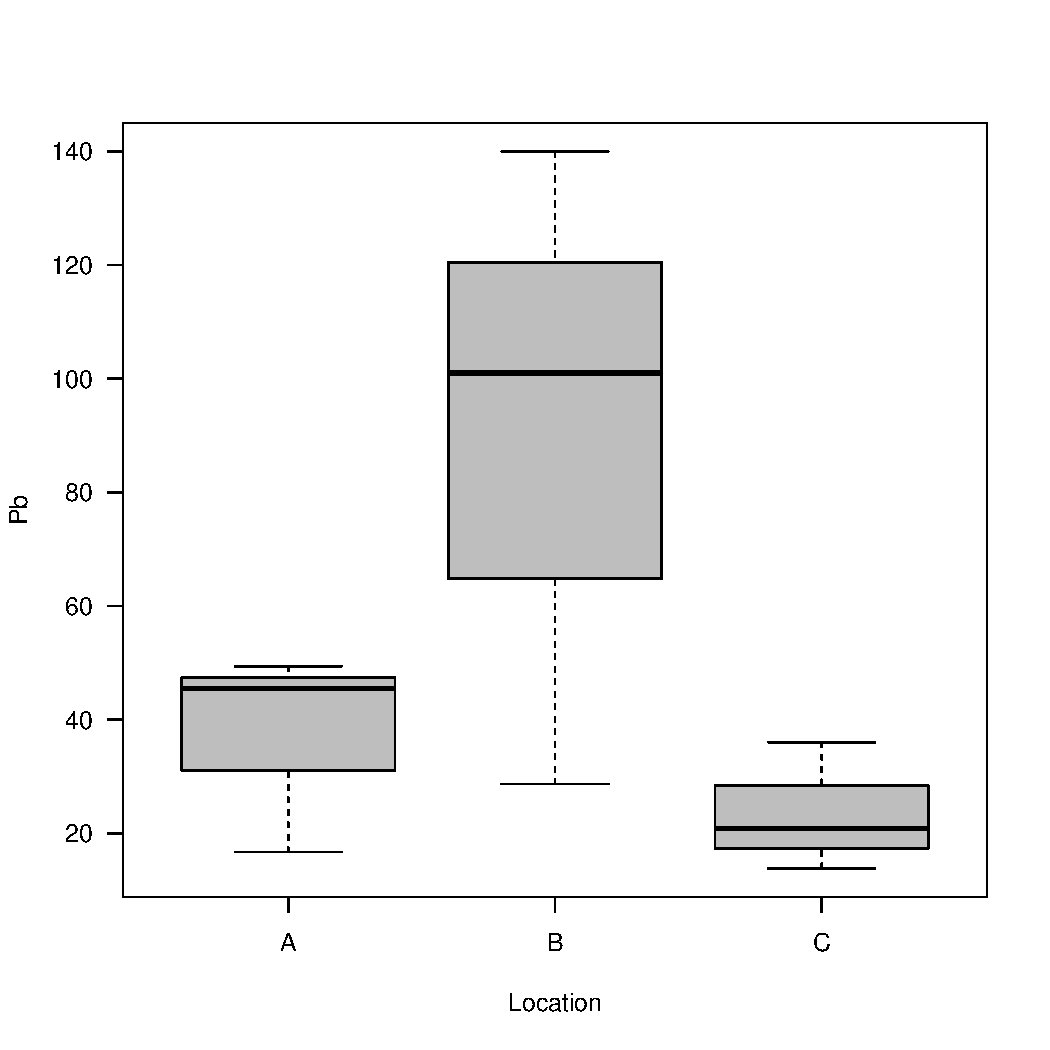
\includegraphics[width=\maxwidth]{figure/boxplot-1} 

\end{knitrout}
\caption{Figure Caption...}
\label{fig.boxplot}
\end{figure}
\begin{knitrout}
\definecolor{shadecolor}{rgb}{0.969, 0.969, 0.969}\color{fgcolor}\begin{kframe}
\begin{alltt}
\hlstd{fakedata.aov} \hlkwb{=} \hlkwd{aov}\hlstd{(Pb} \hlopt{~} \hlstd{Location,} \hlkwc{data}\hlstd{=fakedata)}
\hlkwd{summary}\hlstd{(fakedata.aov)}
\end{alltt}
\begin{verbatim}
##             Df Sum Sq Mean Sq F value Pr(>F)
## Location     2  341.5   170.8   0.356  0.714
## Residuals    6 2879.0   479.8
\end{verbatim}
\end{kframe}
\end{knitrout}
\section{Discussion}

This is the context and interpreations section that relies on some articles, e.g. \cite{struzynska2005role}.
\section{Conclusion}

\bibliography{Report}

\end{document}

